\documentclass[convert]{standalone}

\usepackage{tikz}

\usetikzlibrary{automata}
\usetikzlibrary{positioning}
\usetikzlibrary{arrows}
\tikzset{node distance=2.5cm,
         every state/.style={semithick},
         initial text={},
         double distance=2pt,
         every edge/.style={draw, ->, auto, semithick} }

\begin{document}
\resizebox{30in}{!}
{ 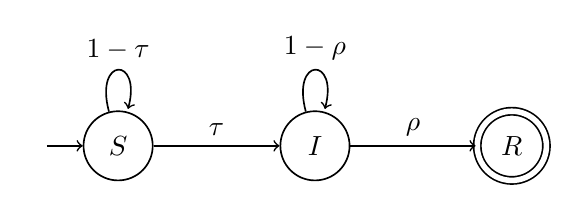
\begin{tikzpicture}
    \node[state, initial] (q1) {$S$};
    \node[state, right of=q1] (q2) {$I$};
    \node[state, accepting, right of=q2] (q3) {$R$};
    \draw (q1) edge[loop above] node {$1-\tau$} (q1);
    \draw (q1) edge node {$\tau$} (q2);
    \draw (q2) edge[loop above] node {$1-\rho$} (q2);
    \draw (q2) edge[] node {$\rho$} (q3);
  \end{tikzpicture} }
\end{document}
